\documentclass[11pt,letterpaper]{article}
\usepackage[lmargin=1in,rmargin=1in,tmargin=1in,bmargin=1in]{geometry}
\usepackage{../style/homework}
\usepackage{../style/commands}
\setbool{quotetype}{true} % True: Side; False: Under
\setbool{hideans}{false} % Student: True; Instructor: False

% -------------------
% Content
% -------------------
\begin{document}

\homework{8: Due 11/09}{I did not attend his funeral, but I sent a nice letter saying I approved of it.}{Mark Twain} 

% Problem 1
\problem{10} Find the least square regression line for the points: $(1, 1), (1,0), (2,3), (3,4)$. Show all your work. \pspace

\sol We have 4 points so that $n= 4$. First, we compute the $x$ and $y$ averages---$\overline{x}$ and $\overline{y}$, respectively. 
	\[
	\begin{aligned}
	\overline{x}&= \dfrac{\sum x_i}{n}= \dfrac{1 + 1 + 2 + 3}{4}= \dfrac{7}{4} \approx 1.75 \\
	\overline{y}&= \dfrac{\sum y_i}{n}= \dfrac{1 + 0 + 3 + 4}{4}= \dfrac{8}{4} \approx 2.00 
	\end{aligned}
	\]
Now we compute $s_x, s_y, r$:
	\begin{table}[!ht]
	\centering
	\begin{tabular}{rrrrrr}
	$x$ & $y$ & $x_i - \overline{x}$ & $(x_i - \overline{x})^2$ & $y_i - \overline{y}$ & $(y_i - \overline{y})^2$ \\ \hline
	$1$ & $1$ & $-0.75$ & $0.5625$ & $-1$ & $1$ \\ 
	$1$ & $0$ & $-0.75$ & $0.5625$ & $-2$ & $4$ \\
	$2$ & $3$ & $0.25$ & $0.0625$ & $1$ & $1$ \\
	$3$ & $4$ & $1.25$ & $1.5625$ & $2$ & $4$ \\ \hline
	& Total: & & $2.75$ & & $10$ 
	\end{tabular}
	\end{table}
Then we have
	\[
	\begin{aligned}
	s_x^2&= \dfrac{1}{n - 1} \sum (x_i - \overline{x})^2= \dfrac{1}{4 - 1} \cdot 2.75= 0.9167 \Longrightarrow s_x= \sqrt{0.9167}= 0.9574 \\
	s_y^2&= \dfrac{1}{n - 1} \sum (y_i - \overline{y})^2= \dfrac{1}{4 - 1} \cdot 10= 3.3333 \Longrightarrow s_y= \sqrt{3.3333}= 1.8257
	\end{aligned}
	\]
Now we also compute the $r$ value:
	\begin{table}[!ht]
	\centering
	\begin{tabular}{rrrrrrr}
	$x$ & $y$ & $x_i - \overline{x}$ & $\frac{x_i - \overline{x}}{s_x}$ & $y_i - \overline{y}$ & $\frac{y_i - \overline{y}}{s_y}$ & $\frac{x_i - \overline{x}}{s_x} \cdot \frac{y_i - \overline{y}}{s_y}$ \\ \hline
	$1$ & $1$ & $-0.75$ & $-0.7833$ & $-1$ & $-0.5477$ & $0.4291$ \\ 
	$1$ & $0$ & $-0.75$ & $-0.7833$ & $-2$ & $-1.0954$ & $0.8581$ \\
	$2$ & $3$ & $0.25$ & $0.2611$ & $1$ & $0.5477$ & $0.1430$ \\
	$3$ & $4$ & $1.25$ & $1.3056$ & $2$ & $1.0954$ & $1.4302$ \\ \hline
	& Total: & &  & & & $2.8604$
	\end{tabular}
	\end{table}
	\[
	r= \dfrac{1}{n - 1} \sum \left( \dfrac{x_i - \overline{x}}{s_x} \right) \left( \dfrac{y_i - \overline{y}}{s_y} \right)= \dfrac{1}{4 - 1} \cdot 2.8604= 0.9534
	\]
Therefore, $r^2= 0.9090$. Finally, we can compute our regression coefficients:
	\[
	b_1= r\, \dfrac{s_y}{s_x}= 0.9534 \cdot \dfrac{1.8257}{0.9574}= 1.818 \quad \text{ and } \quad b_0= \overline{y} - b_1 \overline{x}= 2.00 - 1.818 \cdot 1.75= -1.181
	\]
Therefore, as $\widehat{y}= b_1x + b_0$, we know $\widehat{y}= 1.818x - 1.181$. 





\newpage





% Problem 2
\problem{10} Given the following information below, find the least square regression line. Show all your work. 
	\[
	\begin{aligned}
	n&= 11 \\
	\overline{x}&= 3.45, \quad \sigma_x^2&= 7.073 \\
	\overline{y}&= 6.81, \quad \sigma_y^2&= 5.371 \\
	R&= 0.802
	\end{aligned}
	\] \pspace

\sol Because $\sigma_x^2= 7.073$ and $\sigma_y^2= 5.371$, we know that $\sigma_x= \sqrt{7.073}= 2.6595$ and $\sigma_y= \sqrt{5.371}= 2.3175$. But then\dots
	\[
	\begin{aligned}
	b_1&= R\;\dfrac{\sigma_y^2}{\sigma_x^2}= 0.802\; \dfrac{2.3175}{2.6595}= 0.699 \\[0.3cm]
	b_1&= \overline{y} - b_1 \overline{x}= 6.81 - 0.699 \cdot 3.45= 4.398
	\end{aligned}
	\] \pvspace{0.3cm}
Therefore, as $\widehat{y}= b_1x + b_0$, we know that $\widehat{y}= 0.699x + 4.398$. 





\newpage





% Problem 3
\problem{10} Match each regression coefficient to its corresponding graph. 
	\begin{figure}[!ht]
	\centering
	\begin{minipage}{0.45\textwidth}
	   \centering
	   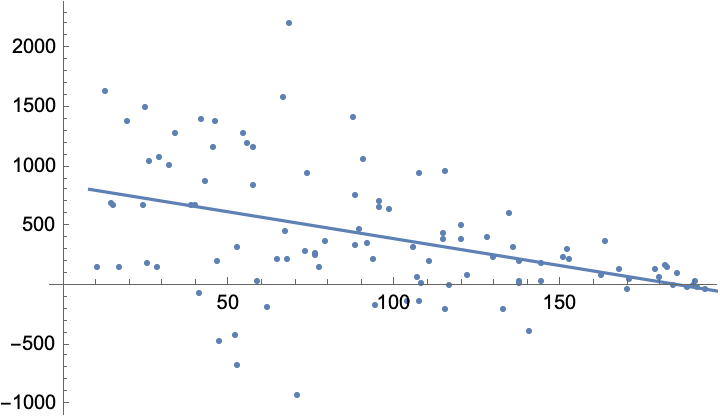
\includegraphics[width=0.9\textwidth]{reg1.png}
	   \caption*{(a)}
	\end{minipage}\hfill
	\begin{minipage}{0.45\textwidth}
	   \centering
	   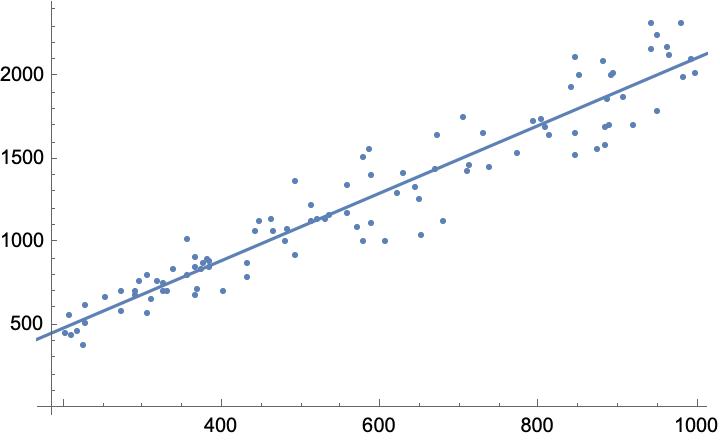
\includegraphics[width=0.9\textwidth]{reg2.png}
	   \caption*{(b)}
	\end{minipage}
	\begin{minipage}{0.45\textwidth}
	   \centering
	   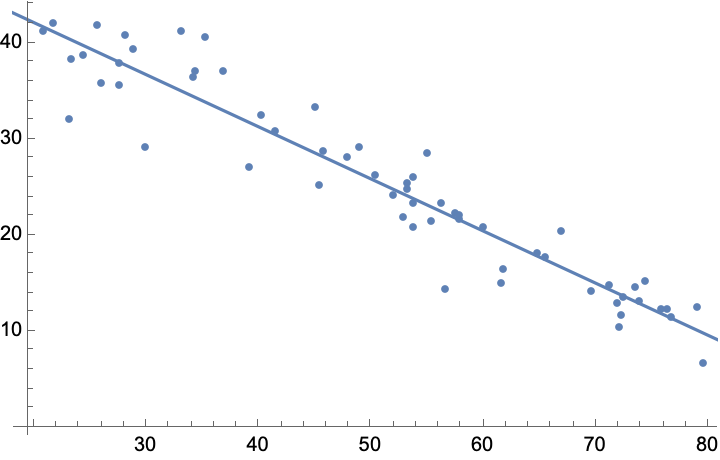
\includegraphics[width=0.9\textwidth]{reg3.png}
	   \caption*{(c)}
	\end{minipage}
	\begin{minipage}{0.45\textwidth}
	   \centering
	   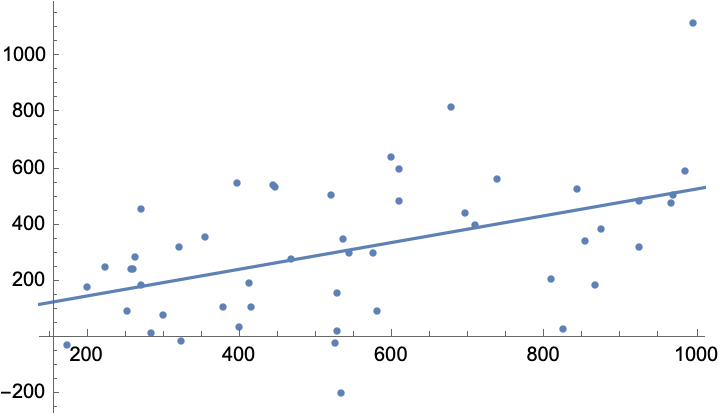
\includegraphics[width=0.9\textwidth]{reg4.png}
	   \caption*{(d)}
	\end{minipage}
	\end{figure}

\begin{enumerate}[(i)]
\item \usol{0.5cm}{(c)}: $R= -0.9529$
\item \usol{0.5cm}{(a)}: $R= -0.4354$
\item \usol{0.5cm}{(d)}: $R= 0.4759$
\item\usol{0.5cm}{(b)}: $R= 0.9573$
\end{enumerate} 





\newpage





% Problem 4
\problem{10} The lengths (in cm) of twenty snakes are taken 6~months after hatching and 2~years after hatching. The data is given below.
	\[
	\begin{aligned}
	(41.2, 163.6), (18.1, 68.9), (42.3, 151.6), (13.2, 43.9), (45.8, 189.5), \\ 
	(42.7, 180.5), (24.4, 92.8), (49.0, 166.), (24.6, 101.1), (18.9, 77.5), \\
	(16.3, 63.6), (36.3, 142.2), (32.2, 124.3), (36.3, 121.), (24.7, 77.8), \\
	(40.1, 139.7), (22.3, 72.8), (42.4, 182.2), (21.4, 73.), (12.3, 53.1)
	\end{aligned}
	\]
A linear regression for this data was found to be $\widehat{y}= 3.9x - 3.1$ with $R= 0.9381$. 
	\begin{enumerate}[(a)]
	\item Was the linear regression a good fit for the data? Explain.
	\item Find the residual for the data point $(41.2, 163.6)$. Was the model under or over prediction for the length of the snake? Explain.
	\item Given this data and model, predict the length of a snake after 2~years that measures 32.7~cm 6~months after hatching. 
	\item Should this model be used to predict the length of a snake which is 65~cm six months after hatching? Explain. 
	\end{enumerate} \pspace

\sol 
\begin{enumerate}[(a)]
\item Observe that $R= 0.9381$ and that $R^2= 0.8800$, both of which (being `close' to 1) are good both indicators that this linear regression is a `good' fit for the data. 

\item We have $\widehat{y}(41.2)= 3.9(41.2) - 3.1= 160.68 - 3.1= 157.58$~cm. Therefore, the residual is $e= y_i - \widehat{y}= 163.6 - 157.58= 6.02$~cm. But then the model has under predicted the length of the snake. 

\item We predict the snake has length $\widehat{y}(32.7)= 3.9(32.7) - 3.1= 127.53 - 3.1= 124.43$~cm. 

\item No, it would \textit{not} be appropriate to use this model to make a prediction for a snake this long so soon after hatching. The model was built using only snakes that were length 12.3~cm to 49.0~cm in length. The length 65~cm is `far' above our 49.0~cm. Therefore, it would be inappropriate to extrapolate that far using our model. 
\end{enumerate}


\end{document}